\documentclass[parskip=full]{scrartcl}
\usepackage[utf8]{inputenc} % use utf8 file encoding for TeX sources
\usepackage[T1]{fontenc}    % avoid garbled Unicode text in pdf
\usepackage[german]{babel}  % german hyphenation, quotes, etc
\usepackage{hyperref}       % detailed hyperlink/pdf configuration
\hypersetup{                % ‘texdoc hyperref‘ for options
pdftitle={SWT1: Lastenheft},%
bookmarks=true,%
}
\usepackage{graphicx}       % provides commands for including figures
\usepackage{csquotes}       % provides \enquote{} macro for "quotes"
\usepackage[nonumberlist]{glossaries}     % provides glossary commands
\usepackage{enumitem}

\makenoidxglossaries
%
% % Glossareinträge
%
\newglossaryentry{Dozent}
{
	name=Dozent,
	plural=Dozenten,
	description={Leiter eines oder mehrerer Seminartypen},
}

\newglossaryentry{Cloud}
{
	name=Cloud,
	plural=Clouds,
	description={Über das Internet zugänglicher Server auf dem Nutzer Daten speichern und abrufen können}
}

\newglossaryentry{Meta-Daten}
{
	name=Meta-Daten,
	plural=Meta-Daten,
	description={Hintergrunddaten zu eigentlichen Daten. Wie das Erstellungsdatum eines Textdokumtens.}
}

\newglossaryentry{Seminarveranstaltung}
{
	name=Seminarveranstaltung,
	plural=Seminarveranstaltungen,
	description={Tatsächlich stattfindende Lehrveranstaltung (z.B. \enquote{Schöner Malen -- Anfängerkurs, Sommer 2014})}
}

\newglossaryentry{Computer}
{
	name=Computer,
	description={Gerät zur Verarbeitung zur Daten, das die Daten einlesen, verarbeiten, speichern und ausgeben kann}
}

\title{SWT1: Lastenheft}
\author{Lennart Moritz, 2062822}

\begin{document}

\maketitle

%
% % Hinweise - sollen nicht im endgültigen Dokument erscheinen, daher vor der Abgabe löschen!
%
\section{Vorwort}
Die Dokumentation der Pakete ist häufig lesenswert.
Insbesondere bei den Paketen hyperref und scrguide (KOMA-Script).
Wer TeXLivei per Kommandozeile benutzt kann einfach texdoc scrguide aufrufen.
Windows-Benutzer, die noch nie mit Latex gearbeitet haben, können sich alternativ MikTex anschauen; Mac-Benutzer MacTex.

Zum Erzeugen eines PDFs aus den LATEX-Sourcen empfehlen wir einen Wrapper wie latexmk\footnote{\url{https://www.ctan.org/tex-archive/support/latexmk}} oder einen Editor wie TeXStudio\footnote{\url{http://www.texstudio.org/}} zu verwenden.
Dieser übernimmt beispielsweise das mehrfache Ausführen von pdflatex, wo es notwendig ist.

Legen Sie für dieses Dokument ein neues Verzeichnis in Ihrem Git an, zum Beispiel \texttt{image.lastenheft} und speichern Sie alle benötigten Dateien darin.
Speichern Sie keine von Latex generierten Dateien (außer dem PDF) im Git.
Dies geschieht über die mitgelieferte \texttt{.gitignore}.
Sie können aber auch Ihre persönliche \texttt{.gitignore} bei Bedarf erweitern.

\section{Technisches Schreiben}

Technisches Schreiben ist wichtig für alle Arten von technischen und wissenschaftlichen Dokumenten, also auch im PSE und in der Bachelorarbeit.
Es bedeutet vor allem eine präzise Ausdrucksweise und widerspricht dabei einigen Regeln, die man im Deutschunterricht gelernt hat.
Ein paar praktische Tipps (aus den PSE-Dokumenten von Prof. Snelting):
\begin{itemize}[nosep]
\item Vermeide Adjektive.
      Oft (nicht immer) sind sie unnötig oder ein schlechter Ersatz für einen ungenauen Begriff.
\item Nebensatzkonstruktionen vermeiden; Hauptsätze verwenden!
\item Definiere Begriffe klar und verwende keine Synonyme.
      Synonyme lassen offen, ob genau das gleiche gemeint ist oder nur etwas ähnliches.
      Definiere spezielle Begriffe, z.B. \gls{Computer}, in einem Glossar und verweise im Dokument entsprechend darauf.
\item Abkürzungen sollten bei der ersten Verwendung (EV) ausgeschrieben werden.
      Nach der EV reicht dann die Kurzform.
\item Versuche konkrete Zahlen und Namen anzugeben.
      Vermeide ungenaue Ausflüchte wie: meistens, viele, oft, möglichst, üblich, jemand, manche.
\item Viele kurze Sätze sind einfacher zu verstehen als wenige lange Sätze.
\item Beispiele machen das Endprodukt greifbarer.
\item Illustrationen minimalistisch halten (z.B. IKEA Bauanleitung).
      Eine Information, ein Bild.
      Lieber mehrere ähnliche Bilder als ein komplexes Bild.
\item Vermeide Wiederholung, stattdessen Referenzen benutzen.
      Wiederholungen haben oft subtile Unterschiede, was zu Unklarheit und Verwirrung führt.
      Bei Änderungen wird oft vergessen, dass Wiederholungen auch angepasst werden müssen.
\item Versionskontrolle ergibt auch für technische Texte Sinn und nicht nur für Code.
\end{itemize}

%
% % Hier beginnt die Gliederung des Lastenhefts
%
\section{Zielbestimmung}
Die Pear Corp soll mit dem Produkt in die Lage versetzt werden, Nutzern eine Applikation zum Anwenden von Kunstfiltern auf aus dem Internet bezogenen Bildern zu bieten. Diese Bilder sollen automatisch aus dem Internet geladen werden und nach der Bearbeitung lokal oder auf Pear Corp Servern gespeichert werden können.

\section{Produkteinsatz}

Das Produkt dient der Beschaffung, dem Anwenden von Filtern, der Komprimierung und Speicherung von Bildern. Es soll als Anwendung Lokal auf dem \gls{Computer} des Nutzers ausgeführt werden.

Zielgruppe: Endbenutzer mit Interesse für nicht-professionelle Bildbearbeitung.

Plattform: PC mit Windows XP, Mac OS 10.9.5, Ubuntu 14.04 LTS oder jeweiligem Nachfolger-Betriebssystem

\section{Funktionale Anforderungen}
\begin{itemize}[nosep]
\item[FA10] Es wird eine Startseite für verschiedene Vorgehen angezeigt werden.
\item[FA20] Es gibt ein Vorgehen zur reinen Bildersuche.
	\item[FA21] Die Funktion aus /FA20/ ist in folgenden Punkten konfigurierbar: 
	Anzahl, Nutzungsrechte, Dateiformat und Größe der zu suchenden Bilder.
\item[FA30] Es gibt ein Vorgehen zur Anzeige der letzten Bildern.
	\item[FA31] Das Anzeigen der letzten Bilder öffnet eine Übersicht aller geladenen Bilder.
	\item[FA32] Die Nutzungsrechte der angezeigten Bilder werden dem Nutzer über eine Farbskala angezeigt.
\item[FA40] Es gibt ein Vorgehen zur Bildersuche mit automatischer Komprimierung der gefunden Bilder.
	\item[FA41] Die Funktion aus /FA40/ ist in folgenden Punkten konfigurierbar: 
	Anzahl, Nutzungsrechte, Dateiformat und Größe der zu suchenden Bilder.
\item[FA50] Die (Sub-)Domänen in denen nach Bildern gesucht wird sind Einstellbar.
\item[FA60] Gefundene Bilder können unter Angabe eines Speicherorts lokal oder auf dem Pear Corp Zentralserver gespeichert werden.
\end{itemize}

\section{Produktdaten}
\begin{itemize}[nosep]
\item[PD10] Es sind Meta-Daten der heruntergeladenen Bilder zu speichern.
\item[PD20] Falls ein Bild mit Nutzungsrechten geschützt ist, dann ist die Art der Nutzungsrechte für eine Kategorisierung zu speichern.
\item[PD30] Lädt ein Nutzer ein Bild herunter, sind Daten für die Anzeige der letzten Bilder zu speichern.
\end{itemize}

\section{Nichtfunktionale Anforderungen}
\begin{itemize}[nosep]
\item[NF10] Die Funktion /FA20/ benötigt für 500 Bilder maximal zehn (10) Minuten.
\item[NF20] Die Übersicht aus /FA30/ zeigt maximal 50 Bilder gleichzeitig an.
\item[NF30] Die Dauer des Hochladens von Bildern auf den Zentralserver wächst maximal linear mit der Anzahl der hochzuladenden Bilder.
\item[NF40] Der Zugriff auf den Zentralserver muss von mindestens 100 Nutzern gleichzeitig erfolgen können.
\end{itemize}

\section{Systemmodelle}

\subsection{Szenarien}
\subsubsection{Speichern eines komprimierten Bildes auf dem Zentralserver}
Der Nutzer öffnet die Anwendung und wählt auf der Startseite aus den zur Verfügung stehenden Verfahren die Option \enquote{Bildersuche mit Komprimierung} aus. Es öffnet sich ein Auswahlfenster in dem der Nutzer Suchoptionen angibt. Mit einer Bestätigung seiner Sucheinstellungen werden ihm nach einer Ladezeit eine Reihe von geladenen, komprimierten Vorschaubildern angezeigt. Mit der Maus markiert er ein Bild und und klickt einen Butten zum Hochladen in die \Gls{Cloud} an. Das komprimierte Bild mit den \Gls{Meta-Daten} wird an den Pear Corp Zentralserver gesendet und dort gespeichert.

\subsection{Anwendungsfälle}
\subsubsection{Bildverwaltung}
\begin{center}
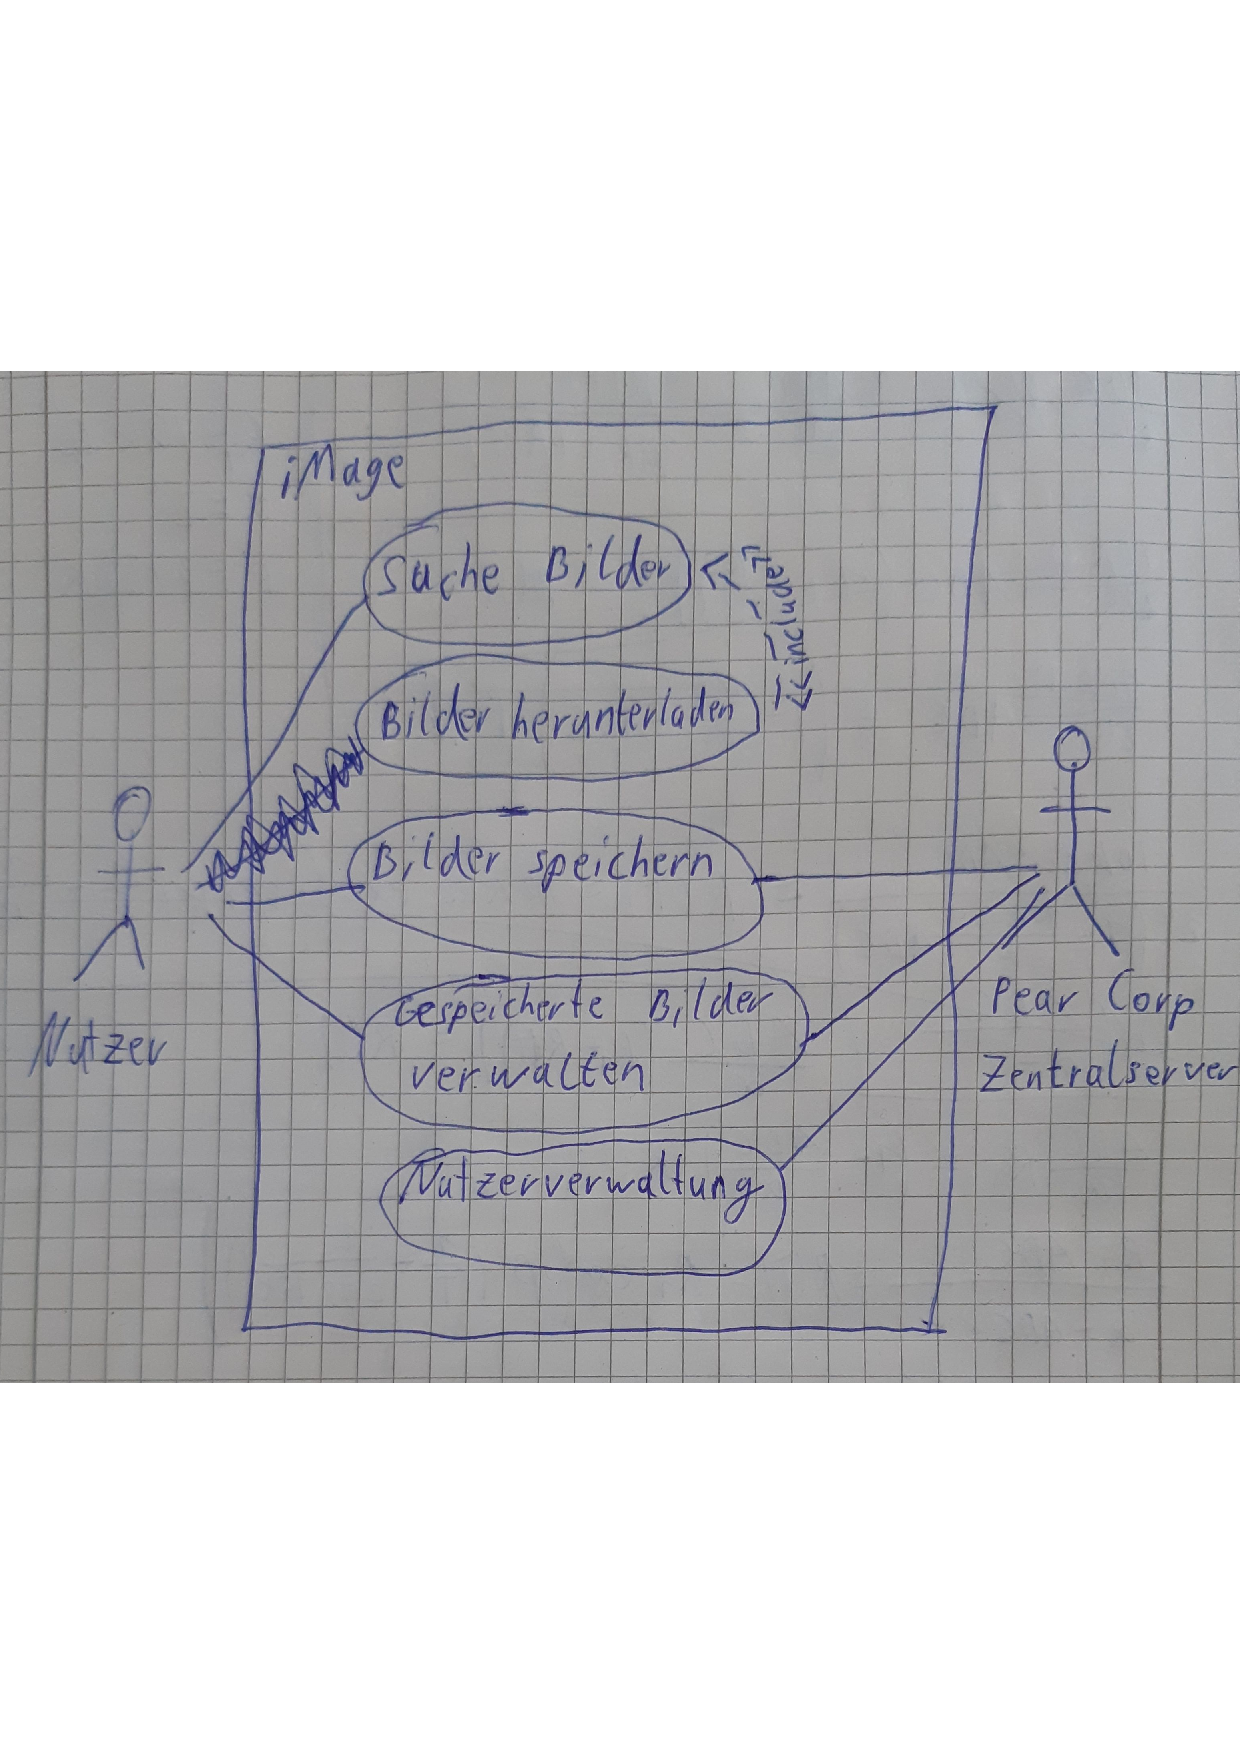
\includegraphics[width=0.8\textwidth]{Anwendungsfalldiagramm.pdf}
\end{center}

Akteure: Nutzer, Pear Corp Zentralserver.

Anwendungsfälle: Suche Bilder, Bilder speichern, Gespeicherte Bilder verwalten, Nutzerverwaltung.

Textuelle Beschreibung:
\begin{itemize}
	\item[Suche Bilder] Der Nutzer lässt sich über das komprimierende oder nicht-komprimierende Verfahren Bilder in einer Vorschau anzeigen. Dabei setzt er Sucheinstellungen und bekommt nach einer Ladezeit die heruntergeladenen und unter Umständen komprimierten Bilder angezeigt, die seiner suche entsprechen.
	\item[Bilder speichern] Der Nutzer markiert aus den geladenen Bildern Elemente zum speichern. Er hat die Option die Bilder lokal zu speichern. Wählt er hingegen aus die Bilder online zu speichern, werden die Bilder von ihm an den Pear Corp Zentralserver gesendet und dieser speichert dann die Bilder.
	\item[Gesp. Bilder verwalten] Sowohl der Nutzer als auch der Zentralserver können die von ihnen gespeicherten Bilder Umbenennen, Löschen und ihre \Gls{Meta-Daten} einsehen.
	\item[Nutzerverwaltung] Der Zentralserver kann Nutzer, die bei ihm Bilder speichern verwalten. Also neue Nutzer anlegen, Nutzerdaten verändern und Nutzer löschen.
\end{itemize}



%
% % Automatisch generiertes Glossar (Latex zwei mal ausführen um Glossar anzuzeigen)
%
%\glsaddall % das sorgt dafür, dass alles Glossareinträge gedruckt werden, nicht nur die verwendeten. Das sollte nicht nötig sein!
\printnoidxglossaries
%Siehe \url{https://en.wikibooks.org/wiki/LaTeX/Glossary}.




\end{document}
